%\part*{Lezione 03/03/2021}
\section{Difficoltà del modello \textit{a shell}}
Torniamo sulle problematiche del modello \textit{a shell}. Prendiamo $\ce{^{130}_{50}Sn_{80}}$, è un pari-pari per cui ci aspettiamo che lo stato fondamentale sia uno $0^+$. I problemi nascono quando cerchiamo di spiegare lo stato $2^+$ a 1 MeV dal fondamentale. Non ho protoni spaiati perché 50 è un numero magico; per quanto riguarda i neutroni, ne mancano 2 per fare il numero magico 82, allora potremmo provare a promuovere un neutrone da uno degli strati inferiori. Tuttavia, poiché il salto dev'essere di 1 MeV non può certo venire da $1g_{9/2}$, per cui supponiamo inizialmente provenga da $3s_{1/2}$: $5\leq j_{3s} + j_{1h}\leq6$, non posso quindi avere $2^+$. Anche se si prova a cercare un altro stato da cui prendere il neutrone non si riesce a trovarne uno che spieghi $J^\pi=2^+$ e il salto di 1 MeV, poiché è sempre necessario \vir{rompere} una coppia di nucleoni (circa 2 MeV). Inoltre, si osserva la presenza di questo stato per ogni nucleo pari-pari con circa $150<A<200$, come in Figura \ref{graf2+} e \ref{graf2+1}.

\begin{figure}[h]
    \centering
    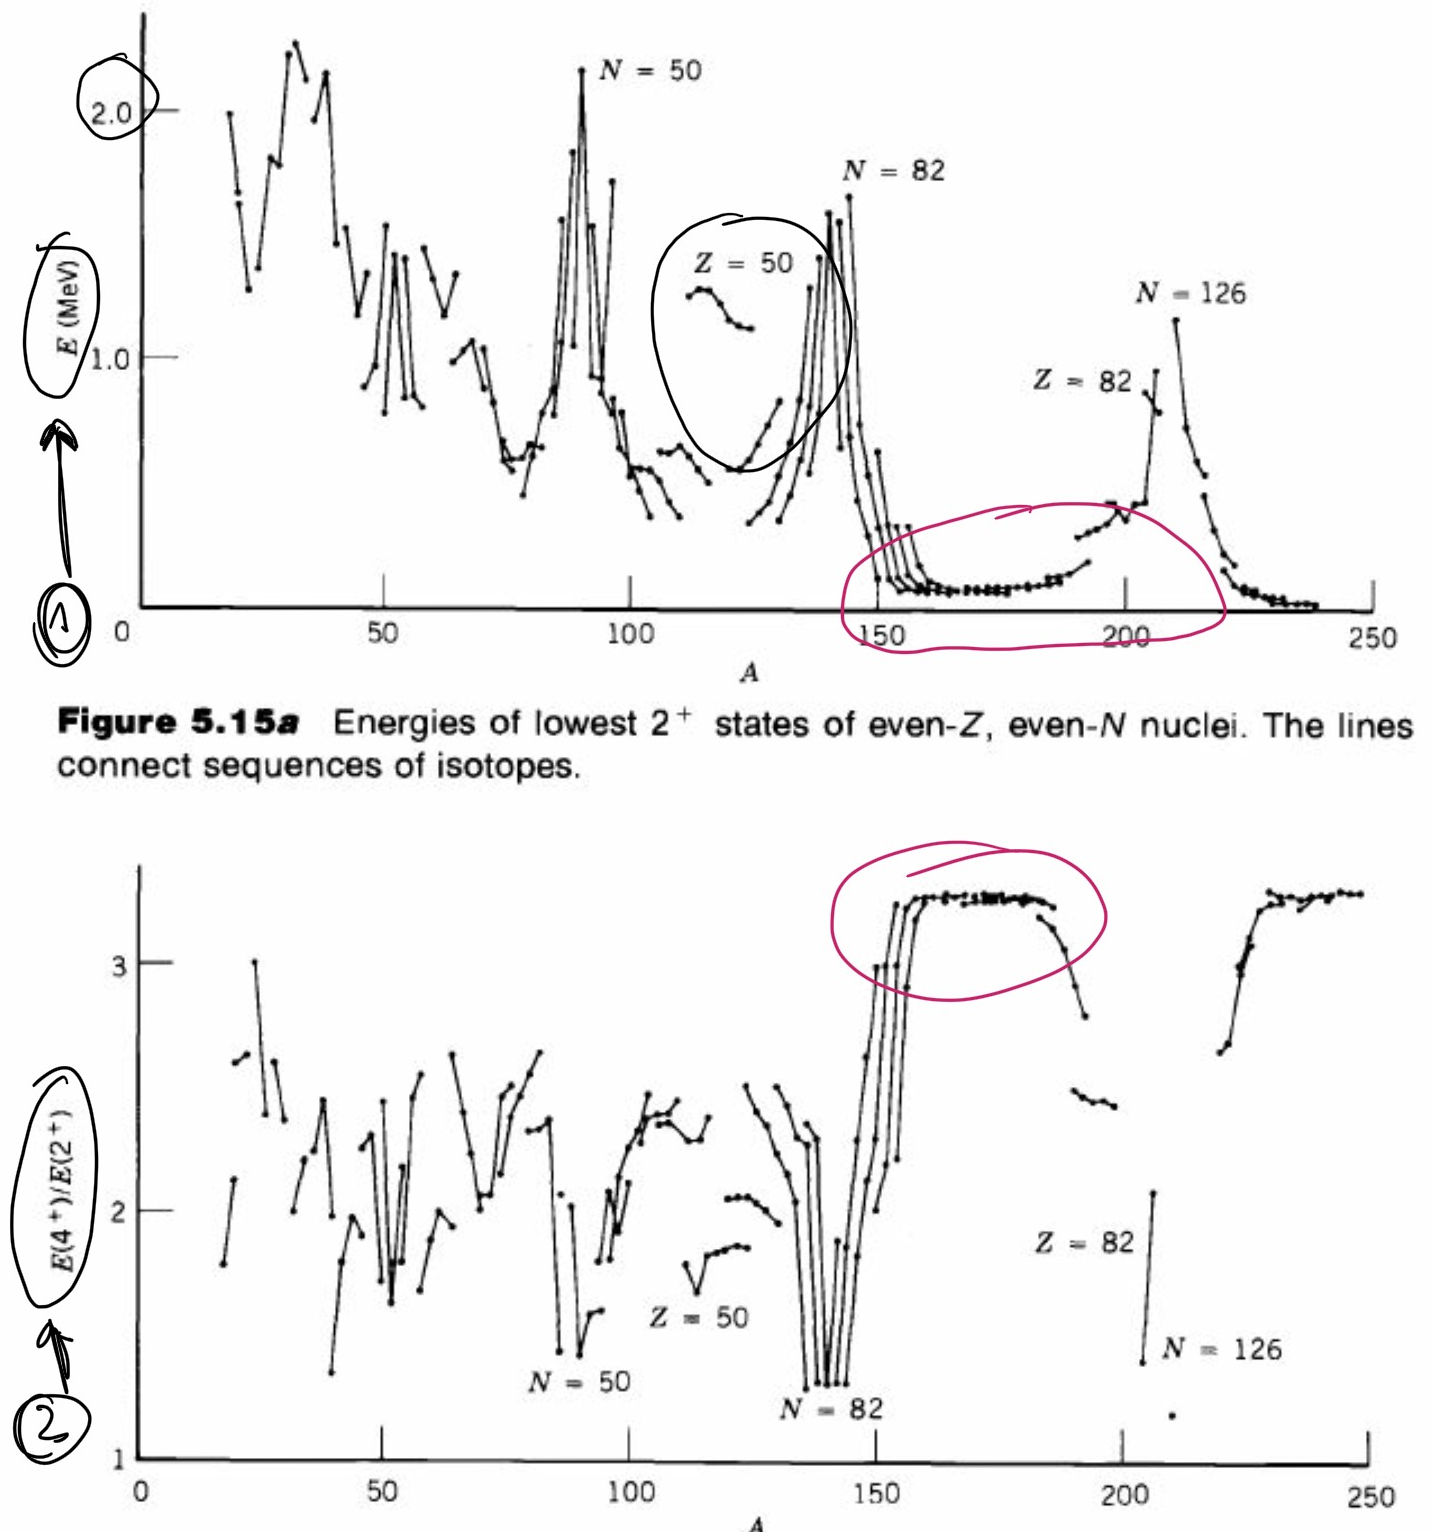
\includegraphics[scale=0.2]{Immagini/150200.png}
    \caption{In basso andamenti del rapporto tra $E(4^+)$ e $E(2^+)$ al variare $A$. Le linee non sono fit, ma collegano semplicemente i dati.}
    \label{graf2+}
\end{figure}
\begin{figure}[h]
    \centering
    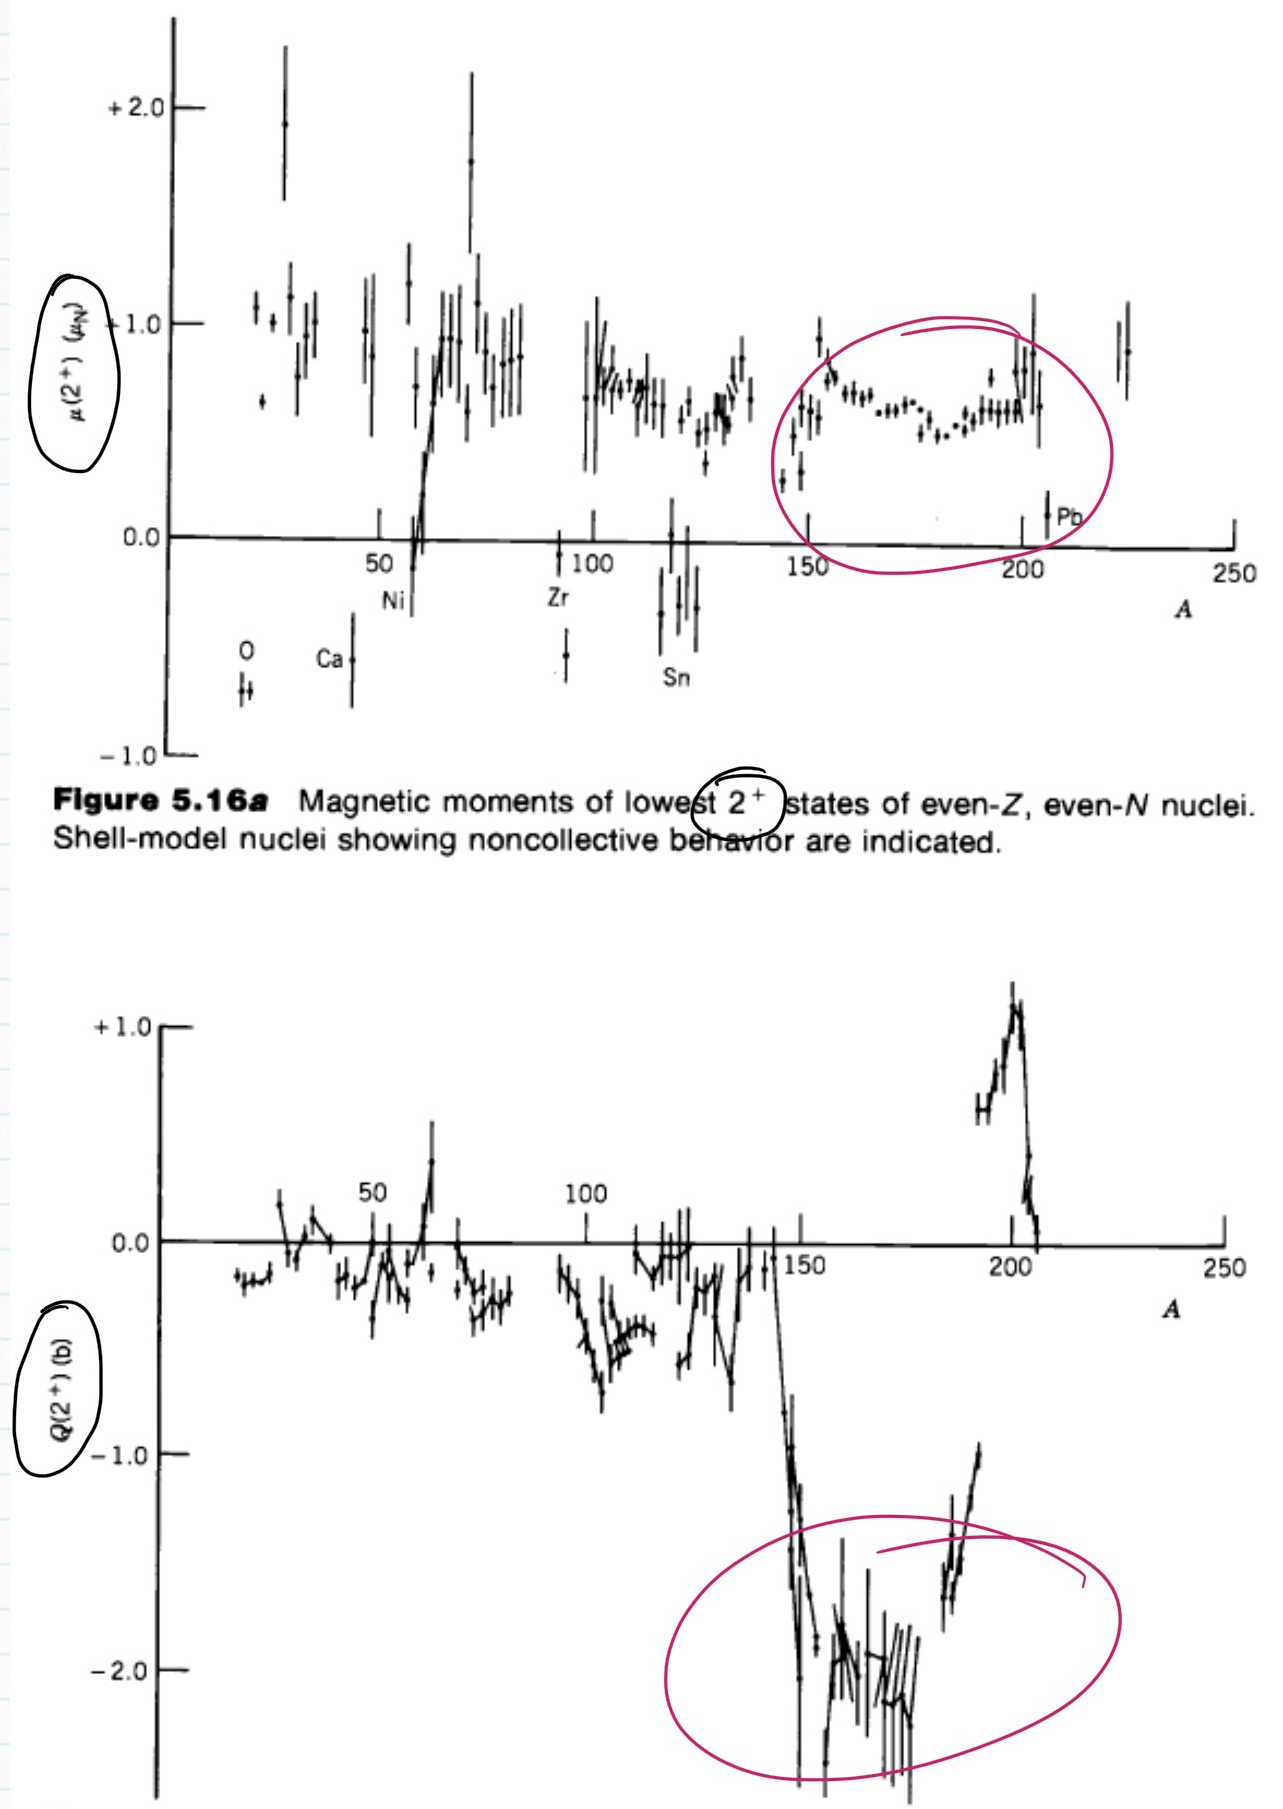
\includegraphics[scale=0.25]{Immagini/150200_2.png}
    \caption{In basso andamento del quadrupolo per lo stato $2^+$ al variare di $A$. Le linee non sono fit, ma collegano semplicemente i dati.}
    \label{graf2+1}
\end{figure}

\subsection{Modello \textit{a goccia} e fononi}
Per spiegare questo comportamento per gli stati eccitati, in particolar modo i momenti di dipolo magnetico e di quadrupolo elettrico, si introduce un nuovo modello detto \textbf{\textit{Liquid Drop Model}}\index{modelli nucleari! a goccia@\textit{a goccia}}: si spiegano gli stati del nucleo come \vir{vibrazioni} della configurazione sferica di equilibrio ed è quindi necessario introdurre stati collettivi (al contrario di quanto prevedeva il modello \textit{a shell}). Pensiamo allora a una \vir{goccia} sferica che si deforma e definiamo $R(t)$ il raggio in funzione del tempo come:
$$R(t) = R_{av} + \sum_{\lambda\geq 1,\; \mu=-\lambda \dots \lambda}\alpha_{\lambda \mu}(t) Y_{\lambda\mu}(\theta,\varphi)$$
con simmetria per riflessione $\alpha_{\lambda\mu} = \alpha_{\lambda\,-\mu}$ e dove abbiamo contato $\lambda=0$ nel raggio medio $R_{av}=R_0\,A^{1/3}$. Per $\lambda=1$ (dipolo) abbiamo una semplice traslazione del centro della sfera (vettore spostamento del $R_{CM}$), mentre per $\lambda = 2$ si ha $Y_{2\mu}$ che è legato a un quadrupolo e quindi a una deformazione della struttura.

\paragraph{Fononi} Possiamo allora prendere $\lambda=2 $ come unità e definire un quanto di energia vibrazionale, il \textbf{fonone}\index{fonone}, che  in questo caso prenderà il nome di fonone di quadrupolo; quindi $0^+ + $ 1 fonone $\lambda=2$, che si porta dietro $Y_{2\mu}$, $\ell =2$ e $\pi=+$:
$$0^+ + 2^+ = 2^+$$
Il $2^+$ è allora il primo stato eccitato vibrazionale del nucleo, anche se l'energia del fonone per ora per noi è un parametro libero. Supponiamo allora di aggiungerne un altro: $\mu = \mu_1 + \mu_2$ e $\mu_i = -2, \dots, 2$, abbiamo quindi $5\cdot 5 = 25$ possibilità. In realtà non è così, ma le possibilità sono solo 15. Guardiamo infatti la Tabella \ref{mumu}: si osserva che per esempio per $\mu=4$ abbiamo una sola possibilità; per $\mu=3$ ne avremmo 2, ma dal momento che il fonone ha \textit{spin} intero la sua funzione d'onda dev'essere simmetrica, quindi le possibilità si riducono a una; per $\mu = 2$ abbiamo 3 possibilità, ma si riducono a 2 e così via. 

\begin{table}[!h]
    \centering
    \begin{tabular}{|c|ccccc|}
        \hline
        \multirow{3}{*}{$\mu_2$} & \multicolumn{5}{c|}{$\mu_1$} \\
        \cline{2-6}
         & -2 & -1 & 0 & 1 & 2 \\
        \hline
        -2 & -4 & -3 & -2 & -1 & 0 \\
        -1 & -3 & -2 & -1 & 0 & 1 \\
        0 & -2 & -1 & 0 & 1 & 2 \\
        1 & -1 & 0 & 1 & 2 & 3 \\
        2 & 0 & 1 & 2 & 3 & 4 \\
        \hline
    \end{tabular}
    \caption{Valori di $\mu=\mu_1+\mu_2$ per 2 fononi di quadrupolo.}
    \label{mumu}
\end{table}
\noindent Tenendo conto quindi dello \textit{spin} del fonone, si arriva a 15 possibilità, ovvero:

\begin{displaymath}
\begin{aligned}
&\ell = 4 & &\mu=-4,\dots,4 & &9 \text{ Possibilità} \\
&\ell = 2 & &\mu=-2,\dots,2 & &5 \text{ Possibilità} \\
&\ell = 0 & &\mu=0 & &1 \text{ Possibilità}\\ 
\hline
& & &\text{Tripletto} & &15 \text{ Possibilità} 
\end{aligned}
\end{displaymath}
\noindent Mi aspetto allora un tripletto $0^+,2^+,4^+$ degenere con energia circa il doppio di quella del $2^+$ di un solo fonone. Ci sono evidenze di questo, per esempio, nel $\ce{^{120}_{52}Te_{68}}$, dove però compaiono\footnote{Non è stato inserito il disegno dei livelli.}, oltre al $2^+$ e al tripletto, il quintetto $2^+,0^+,3^+,4^+,6^+$ (dovuto a 3 fononi) e il $3^-$ (ovvero un ottupolo $\ell=3$).

\paragraph{Bande rotazionali} Con questo modello abbiamo spiegato gli stati $2^+$ e $4^+$, tuttavia non abbiamo ancora chiarito i problemi per i nuclei con $150<A<200$, in particolar modo per quanto riguarda il loro momento di quadrupolo, molto maggiore rispetto a quello dei nuclei con $A<150$ (come in Figura \ref{Q}). \\
Ci aspettiamo quindi nuclei fortemente deformati rispetto alla simmetria sferica dello $0^+$, per cui li descriviamo come ellissodi:
$$R(\theta,\phi) = R_{av}(1+\beta Y_{20}(\theta,\phi))$$
$$\beta = \frac{4}{3}\sqrt{\frac{\pi}{5}} \frac{\Delta R}{R_{av}}$$
dove $\Delta R$ è la differenza tra semiasse maggiore e minore e in prima approssimazione $R_{av}\simeq R_0 A^{\frac{1}{3}}$ è il raggio medio (per cui $V=4\pi R_{av}^3/3$). In base al segno di $\beta$ si ha una figura:
\begin{itemize}
    \item \textbf{prolata}\index{figura!prolata} $\Rightarrow \; \beta >0$, Figura \ref{0303_proobl} a destra.
    \item \textbf{oblata}\index{figura!oblata} $\Rightarrow \; \beta <0$, Figura \ref{0303_proobl} a sinistra.
\end{itemize}
\begin{figure}[h]
    \centering
    \includegraphics[scale=0.7]{Immagini/0303_proobl.png}
    \caption{A sinistra figura oblata, a destra prolata.}
    \label{0303_proobl}
\end{figure}
Possiamo allora calcolare il momento di quadrupolo magnetico nel sistema di riferimento del nucleo:
$$Q_0 = \frac{3}{\sqrt{5\pi}}R^2_{av}Z\beta(1+0.16\,\beta)$$
Tuttavia, se una figura prolata ruota può apparire oblata, per cui se avevamo $Q_0>0$ osserviamo un $Q_0<0$ e questo spiega il valore negativo del momento di quadrupolo. A titolo di esempio, eseguiamo il calcolo per il $2^+$:
$$-2\unit{b} \simeq Q = -\frac{2}{7} Q_0 \; \Rightarrow \; Q_0 \simeq -7\unit{b}$$
$$\beta \simeq 0.29$$
Abbiamo quindi un nucleo fortemente deformato. Se questo ruota la sua energia cinetica sarà data da:
$$E_{cin} = \frac{1}{2} I \omega^2=\frac{1}{2}\frac{L(L+1)}{I}$$
dove $I=L/\omega$ è il momento di inerzia del nucleo; se $L$ aumenta cresce l'energia cinetica, allora ci aspettiamo delle \textbf{bande rotazionali}\index{bande rotazionali} associate ai livelli energetici:
\begin{displaymath}
\begin{aligned}
\text{St}&\text{ato} & &E_{cin} \\
\hline
&0^+ & &0 \\
&2^+ & 6&\frac{\hbar^2}{2I} \\
&4^+ & 20&\frac{\hbar^2}{2I} \\
&\vdots & \vdots&
\end{aligned}
\end{displaymath}
\begin{figure}[h]
    \centering
    \includegraphics[scale=0.6]{Immagini/0303_liv.png}
    \caption{Livelli energetici dell'afnio.}
    \label{0303_livel}
\end{figure}
\noindent Vediamo come esempio\footnote{L'afnio è importante perché il suo decadimento viene utilizzato in fisica medica.} $\ce{^{176}_{72}Hf_{104}}$, i cui livelli\footnote{Per i calcoli abbiamo usato $\hbar^2/2I \sim 88/6 \sim 14.7$ keV} sono riportati in Figura \ref{0303_livel}:
\begin{displaymath}
\begin{aligned}
E(2^+)&= 6\frac{\hbar^2}{2I}\sim 88\, \mbox{keV} \\
E(4^+)&= 20\frac{\hbar^2}{2I}\sim 293\, \mbox{keV} \\
E(6^+)&= 42\frac{\hbar^2}{2I}\sim 621\, \mbox{keV} \\
E(8^+)&= 72\frac{\hbar^2}{2I}\sim 1064\, \mbox{keV} \\
\Rightarrow \frac{E(4^+)}{E(2^+)}&= 3.33
\end{aligned}
\end{displaymath}
L'ultimo risultato è interessante dal momento che è il valore esatto per i rapporti energetici del $\ce{^{164}_{68}Er_{96}}$. Dunque il modello riproduce con ottimo accordo le osservazioni.


\chapter{Decadimenti}
Passiamo a questo punto alla descrizione dei decadimenti $\beta,\alpha$ e $\varepsilon$.
\section{Decadimento $\beta$}
Esistono tre tipologie di \textbf{decadimento} $\beta$:
\begin{itemize}
    \item $\beta^-$: decadimento di un neutrone.
    \item $\beta^+$: decadimento di un protone.
    \item $\varepsilon$: cattura elettronica da parte di un protone.
\end{itemize}
\noindent Abbiamo quindi:
\begin{displaymath}
\begin{aligned}
&\beta^- & \ce{^A_ZX_N}&\to \ce{^A_{Z+1}Y_{N-1}} + e^- + \bar{\nu}_e & n&\to p + e^- + \bar{\nu}_e \\
&\beta^+ & \ce{^A_ZX_N}&\to \ce{^A_{Z-1}Y_{N+1}} + e^+ + \nu_e & p &\to n + e^+ + \nu_e \\
&\varepsilon & \ce{^A_ZX_N} + e^-&\to \ce{^A_{Z-1}Y_{N+1}}  + \nu_e & p+e^- &\to n + \nu_e
\end{aligned}
\end{displaymath}
dove abbiamo separato i processi nucleari da quelli base (che avvengono nel nucleo). Per capire se questi sono\footnote{Con \textit{permessi} e \textit{proibiti} si intende rispettivamente \vir{probabili} e \vir{poco probabili}.} \textit{permessi} o \textit{proibiti} è necessario calcolare il $Q$-\textit{value} $Q=\sum T_i$; possiamo momentaneamente approssimare $m_{\nu}\simeq 0$ MeV e $m_e \simeq 0.5$ MeV, ma dobbiamo considerare $m_n \not \simeq m_p$ per cui $m_n - m_p \simeq 1.3$ MeV: si osserva immediatamente che $m_n>m_p$ implica $\beta^-$ \textit{permesso} ($Q>0$) e $\beta^+$ \textit{proibito} ($Q<0$). Dunque, il protone se libero non decade\footnote{Anche in questo caso si intende che i tempi di decadimento sono \vir{lunghissimi}.}, ma può fare $\beta^+$ solo se è legato e l'energia di legame sia almeno 1.3 MeV.

\subsection{La questione dei neutrini} 
Fino al 1931 non esisteva un modo per identificare la presenza di neutrini, dunque ci si sarebbe aspettati dal grafico del numero di elettroni in funzione dell'energia cinetica degli stessi una funzione a $\delta$ centrata sul valore del $Q$-\textit{value}, perché dalla conservazione dell'energia (trascurando la massa del neutrino) si ha $m(X) = m(Y) + m_e + T_e$ per cui $Q\simeq T_e$.
Tuttavia, quello che invece si osserva è un andamento decrescente come riportato in Figura \ref{0303_ne}.
\begin{figure}[h]
    \centering
    \includegraphics[scale=0.5]{Immagini/0303_nume.png}
    \caption{Distribuzione del numero di neutrini in funzione dell'energia cinetica.}
    \label{0303_ne}
\end{figure}
Inizialmente, si cercò di spiegare questo fatto supponendo che gli elettroni prima di uscire dal campione urtassero contro altri elettroni atomici, ridistribuendo così la loro energia cinetica, ma questo non era esaustivo. Fu Pauli il primo a ipotizzare l'esistenza del neutrino; calcolando il $Q$-\textit{value}:
$$Q = m_n - m_p - m_e - m_\nu \simeq 0.78 \;\mbox{MeV} - m_\nu$$
per cui dalla misura di questo si può ricavare una stima per la massa del neutrino. Il problema è che è estremamente difficile, infatti i dati riportarono $Q = (0.782 \pm 0.013)$ per cui $m_\nu \simeq 0$ entro 13 keV\footnote{Con le misure più recenti si ha $m_\nu \simeq 0$ entro 1 eV}. Dunque, non è una \vir{cattiva} approssimazione quella di trascurare la massa del neutrino rispetto alle altre masse in gioco, a meno che i neutrini non siano i protagonisti del fenomeno in esame. Calcoliamoci\footnote{Procederemo in realtà al calcolo esplicito solo del decadimento $\beta^-$, poiché gli altri sono concettualmente identici.} dunque il $Q$-\textit{value} di questi decadimenti trascurando la massa del neutrino:
$$m_{at} (\ce{_{Z}X}) \equiv m(\ce{^A_ZX_N})+Zm_e - \sum_{i=1}^Z B_i$$
\begin{displaymath}
\begin{aligned}
Q_{\beta^-} &= m_{at}(\ce{_ZX}) - Zm_e + \sum_{i=1}^Z B_i - m_{at}(\ce{_{Z+1}Y}) + (Z+1) m_e - \sum_{i=1}^{Z+1} B_i - m_e= \\
&= m_{at}(\ce{_ZX}) - m_{at}(\ce{_{Z+1}Y}) + \sum_{i=1}^Z B_i - \sum_{i=1}^{Z+1} B_i \simeq \\
&\simeq m_{at}(\ce{_ZX}) - m_{at}(\ce{_{Z+1}Y}) \\
Q_{\beta^+} &= m_{at}(\ce{_ZX}) - m_{at}(\ce{_{Z+1}Y}) - 2m_e \\
Q_{\varepsilon} &= m_{at}(\ce{_ZX}) - m_{at}(\ce{_{Z+1}Y}) - B_n
\end{aligned}
\end{displaymath}
dove abbiamo fatto l'approssimazione $Z\sim Z+1$ poiché stiamo considerando atomi con $Z$ molto \vir{alto} e dove abbiamo definito $B_n$ la binding energy per $n$ numero di shell ($n = k,L,\dots$). Vediamo alcuni esempi:
\begin{displaymath}
\begin{aligned}
&\text{Decadimento} & &Q & \tau_{\frac{1}{2}}& \\
\hline
&\ce{^{23}Ne} \betamin \ce{^{23}Na} & &4.38 & 38&\,\mbox{s} \\
&\ce{^{99}Tc} \betamin \ce{^{99}Ru} & &0.29 & 2\cdot 10^5&\,\mbox{y} \\
&\ce{^{25}Al} \betaplu \ce{^{25}Mg} & &3.26 & 7.2&\,\mbox{s} \\
&\ce{^{134}I} \betaplu \ce{^{134}Te} & &2.14 & 4.2&\,\mbox{d} \\
\end{aligned}
\end{displaymath}
Da queste osservazioni sembra che il periodo di dimezzamento sia scorrelato dal $Q$-\textit{value}, coprendo parecchi ordini di grandezza. Fermi riuscì a spiegare questo andamento.